%
% 04001-W.tex -- Wavelet transform
%
% (c) 2019 Prof Dr Andreas Müller, Hochschule Rapperswil
%
\documentclass[tikz]{standalone}
\usepackage{amsmath}
\usepackage{times}
\usepackage{txfonts}
\usepackage{pgfplots}
\usepackage{csvsimple}
\usetikzlibrary{arrows,intersections,math}
\begin{document}
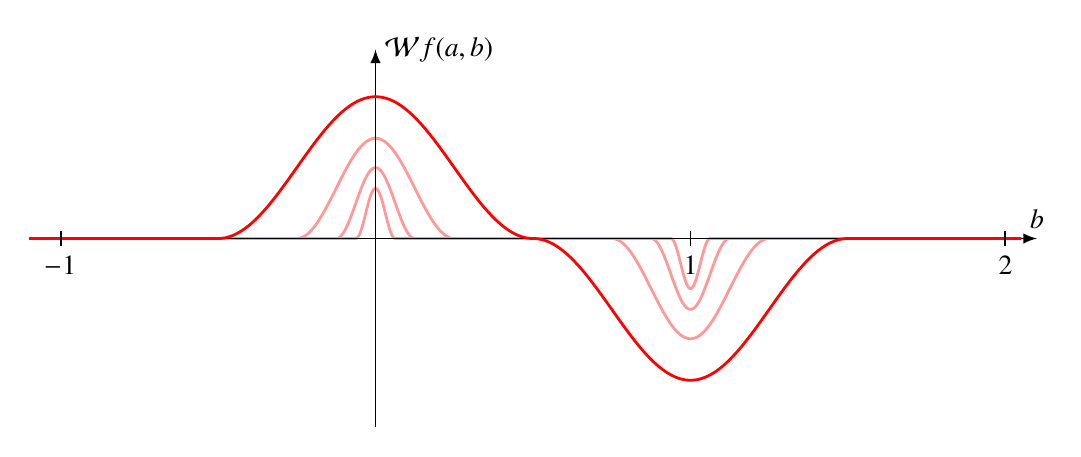
\begin{tikzpicture}[>=latex,scale=4]
\def\vs{1}

\foreach \a in {0.25,0.125,0.0625}{
\draw[color=red!40,line width=1pt]
	(-1.1,0)--({-\a},0)--
	plot[domain={-\a}:{\a},samples=100]
		({\x},{\vs*\a*(1+cos((\x/\a)*180))/(sqrt(\a)*3.1415)})
	--
	plot[domain={1-\a}:{1+\a},samples=100]
		({\x},{-\vs*\a*(1+cos(((1-\x)/\a)*180))/(sqrt(\a)*3.1415)})
	--(2.05,0);
}
\draw[->,line width=0.7pt] (-1.1,0)--(2.1,0)
	coordinate[label={$b$}];
\draw[->,line width=0.7pt] (0,-0.6)--(0,0.6)
	coordinate[label={right:$\mathcal{W}f(a,b)$}];
\def\a{0.5}
\draw[color=red,line width=1pt] (-1.1,0)--(-0.5,0)--
	(-1.1,0)--({-\a},0)--
	plot[domain={-\a}:{\a},samples=100]
		({\x},{\vs*\a*(1+cos((\x/\a)*180))/(sqrt(\a)*3.1415)})
	--
	plot[domain={1-\a}:{1+\a},samples=100]
		({\x},{-\vs*\a*(1+cos(((1-\x)/\a)*180))/(sqrt(\a)*3.1415)})
	--(2.05,0);

\draw[line width=0.7pt] (-1,-0.025)--(-1,0.025);
\draw[line width=0.7pt] (1,-0.025)--(1,0.025);
\draw[line width=0.7pt] (2,-0.025)--(2,0.025);
\node at (-1,-0.025) [below] {$-1$};
\node at (1,-0.025) [below] {$1$};
\node at (2,-0.025) [below] {$2$};
\end{tikzpicture}
\end{document}
